%--------------------------------------------------------------------------------------------
%   YART thesis "Implementation" chapter definition.
%--------------------------------------------------------------------------------------------

\chapter{Implementation} \label{ch:Implementation}

Before delving into the implementation of a ray tracing engine, certain considerations should be made, which will define the entire development workflow.
One such example is the choice of a coordinate system, that will affect the order of mathematical calculations.
Coordinate systems provide a standardized way of specifying locations and orientations of objects within a multi-dimensional environment.
In the context of two-dimensional computer graphics, the system typically consists of a X-axis pointing from left to right, and a Y-axis pointing upwards.
When adding the third coordinate however, the developer has a choice as to whether the Z-axis should point out of, or into the virtual screen, away from the viewer.
These two system types are respectively referred to as the right-handed coordinate system (RHS), and the left-handed coordinate system (LHS) (see \cref{fig:Implementation/coordinate_system}).
The names of these systems derive from the \textit{right-hand rule}, which is a convention used for determining the orientation of axes in three-dimensional space \supercite{RightHandRule}. 

\vfill
\begin{figure}[!ht]
    \centering

    \begin{subfigure}{.4\textwidth}
        \centering

        \begin{tikzpicture}[scale=1.15, every node/.style={scale=1.15}]
            \draw[-{Latex[length=3mm]}, color=axis_red, very thick]   (0, 0) -- (2, -0.7);
            \draw[-{Latex[length=3mm]}, color=axis_green, very thick] (0, 0) -- (0, 2);
            \draw[-{Latex[length=3mm]}, color=axis_blue, very thick]  (0, 0) -- (-1.6, -0.9);
            \node[color=axis_red] (x) at (2.05, -0.4) {\textbf{x}};
            \node[color=axis_green] (y) at (-0.3, 1.95) {\textbf{y}};
            \node[color=axis_blue] (y) at (-1.7, -0.6) {\textbf{z}};
        \end{tikzpicture}
        \caption{}
    \end{subfigure}%
    \begin{subfigure}{.4\textwidth}
        \centering
        
        \begin{tikzpicture}[scale=1.25, every node/.style={scale=1.25}]
            \draw[-{Latex[length=3mm]}, color=axis_red, very thick]   (0, 0) -- (2, -0.7);
            \draw[-{Latex[length=3mm]}, color=axis_green, very thick] (0, 0) -- (0, 2);
            \draw[-{Latex[length=3mm]}, color=axis_blue, very thick]  (0, 0) -- (1.6, 0.9);
            \node[color=axis_red] (x) at (2.05, -0.4) {\textbf{x}};
            \node[color=axis_green] (y) at (-0.3, 1.95) {\textbf{y}};
            \node[color=axis_blue] (y) at (1.5, 1.12) {\textbf{z}};
        \end{tikzpicture}
        \caption{}
    \end{subfigure}

    \caption[RHS and LHS coordinate systems]{RHS (a) and LHS (b) coordinate systems.}
    \label{fig:Implementation/coordinate_system}
\end{figure}
\vfill

Both the RHS and LHS are commonly utilized in commercial rendering software.
While developing YART, the left-handed coordinate system has been used, solely based on personal preference. 
This information is important to keep in mind, as the choice of a system determines the definition and implementation of projections, and various matrix operations, used throughout a ray tracing engine. 

\section{Ray Definition}

The fundamental piece of any ray tracing engine is undeniably the concept of \textit{rays}.
In mathematics, a ray can be defined as a straight line extending infinitely in one direction from a specific starting point. 
It is therefore characterized by its origin point, and a unit vector denoting the directions it's facing.
Rays can be conceptualized across any number of dimensions, however for the specific application of ray tracing, we will only focus on three-dimensional rays.

Let's consider a ray with an origin point $ \bm{P} $, extending infinitely in the direction of a vector $ \bm{\hat{v}} $.
To sample a specific point along this ray, we define a function $ \bm{r} $
%
\begin{equation}
    \bm{r}(t) = \bm{P} + t\bm{\hat{v}}
    \label{eq:Implementation/RayDefinition/ray}
\end{equation}
%
It returns all possible points on the ray, which are $ t $ units apart from its origin.
Knowing the distance from the ray's origin to the closest object hit along its path, function $ \bm{r} $ will enable us to find the exact point of collision on the object's surface.
For this purpose, it's important to make the direction vector $ \bm{\hat{v}} $ an unit vector, as a vector of length different than $ 1 $ would scale the distance proportionately, ultimately resulting in inaccurate calculations. 

In the code, we can define a ray as a lightweight structure containing two three-dimensional vector members, representing the ray's origin and direction (see \cref{lst:Implementation/RayDefinition/ray}).
This structure can later be extended with related operations, such as testing for ray-object intersections or reflecting of a given surface.

\vfill
\lstinputlisting[
    xleftmargin=1.5em, 
    caption={[Ray structure definition]
        Ray structure definition.},
    label={lst:Implementation/RayDefinition/ray}
]{include/listings/ListingRay.cpp}
\vfill

\section{Ray Generation and The Camera}

To render images using ray tracing methodology, generally means to trace a single ray for every pixel in the output image.
The color seen it the direction of those rays, is what defines the final color of their respective pixels. 
This initial phase of calculating ray directions for every image pixel, is often referred to as the \textit{ray generation} step of a ray tracing engine.
Ray generation in YART can be divided into four stages:
\begin{enumerate}
    \item defining and querying camera properties,
    \item computing a screen-space-to-camera-space transformation matrix,
    \item calculating individual ray directions using the matrix,
    \item caching the calculated direction vectors.
\end{enumerate}

\subsection{Camera Definition}

Before we can generate a ray, we first need to explain the basic concept behind a \textit{camera}.
Sometimes referred to as the \textit{eye}, a camera is the engine's virtual viewpoint, giving the ability to "see" into a digital environment.
At its core, it's used to generate rays for each pixel in the rendered image.
It is primarily represented by its position in world-space, a viewing direction (or \textit{look-at vector}), and the camera's field of view (FOV).
A camera's field of view represents the angular extent of the scene captured in the output image. 
FOV might be expressed in one of three different ways, as it can be measured horizontally, vertically, or diagonally.
The difference between them is significant, impacting the calculations made while defining a projection matrix.
In YART, horizontal measurement is used to determine camera's field of view.

The camera can be though of as a viewing context for rendering a scene.
Rays will be cast originating from the camera's position and traced in the direction it is facing, offset by \textit{screen-space} coordinates of subsequent image pixels.
Screen-space coordinates generally refer to a two-dimensional coordinate system that represents the positions of pixels on a screen.
In the context of ray tracing, the screen can be represented as an image, positioned at a specific distance from the camera's origin. 
This concept is otherwise knows as the camera's \textit{image plane} or \textit{viewport}.
The image plane pixel positions in camera's local-space (or \textit{camera-space}) is what will let us determine ray directions for a particular pixel. 
\cref{fig:Implementation/RayGeneration/iamge_plane} illustrates a camera with the center of its viewport positioned at the end of the look-at-vector.  

\vfill
\begin{figure}[!ht]
    \centering

    % Top margin
    \vspace{1cm}

    \begin{tikzpicture}[scale=1.0, every node/.style={scale=1.0}]
        % Plane inner lines
        \draw[-, color=gray, thin] (6.25, 2.42) -- (9.55, 1.6);
        \draw[-, color=gray, thin] (6.25, 1.9) -- (9.46, 0.78);
        \draw[-, color=gray, thin] (6.25, 1.38) -- (9.4, -0.05);
        \draw[-, color=gray, thin] (6.25, 0.9) -- (9.35, -0.85);
        \draw[-, color=gray, thin] (6.25, 0.4) -- (9.3, -1.62);

        \draw[-, color=gray, thin] (6.6, 2.92) -- (6.57, -0.35);
        \draw[-, color=gray, thin] (7, 2.87) -- (6.95, -0.63);
        \draw[-, color=gray, thin] (7.5, 2.82) -- (7.4, -0.98);
        \draw[-, color=gray, thin] (8.08, 2.7) -- (7.92, -1.35);
        \draw[-, color=gray, thin] (8.75, 2.65) -- (8.53, -1.82);

        % Pixel diagonals 
        \draw[-, color=gray, ultra thin] (7.95, -0.72) -- (8.6, -0.43);

        % Plane outer lines
        \draw[-, color=darkgray, very thick] (6.25, 2.97) -- (9.6, 2.53)
        -- (9.25, -2.35) -- (6.25, -0.1) -- (6.25, 2.97) -- (9.6, 2.53);
        \node[color=darkgray, rotate=-7] (x) at (7.9, 3.1) {\textbf{Image Plane}};

        % Looking direction vector
        \draw[-{Latex[length=3mm]}, color=axis_blue, very thick] (0.037, 0.005) -- (7.45, 0.835);
        \node[color=axis_blue, rotate=6.6] (x) at (4.55, 0.75) {\textbf{Look-at Vector}};

        % Ray 
        \draw[-{Latex[length=3mm]}, color=axis_red, very thick] (0.037, 0.005) -- (12, -0.855);
        \node[color=axis_red, rotate=-4] (x) at (11, -0.5) {\textbf{Ray}};

        % Camera to plane lines
        \draw[-, color=darkgray, thin] (0, 0) -- (6.235, 2.982);
        \draw[-, color=darkgray, thin] (0, 0) -- (9.6, 2.53);
        \draw[-, color=darkgray, thin] (0, 0) -- (9.25, -2.366);
        \draw[-, color=darkgray, thin] (0, 0) -- (6.25, -0.11);

        % Overlays over the ray
        \draw[{Round Cap[]}-{Round Cap[]}, color=gray, thin] (8.883, -0.5862) -- (9.15, -0.737);
        \draw[{Round Cap[]}-{Round Cap[]}, color=gray, thin] (8.593, -0.54) -- (8.583, -0.737);
        \draw[-, color=darkgray, very thick] (9.6, 2.53) -- (9.25, -2.35);

        % Pixel diagonals 
        \draw[-, color=gray, ultra thin] (7.973, -0.075) -- (8.57, -1.143);

        % Camera origin
        \node[fill=darkgray, circle, inner sep=0pt, minimum size=2.5mm] (c) at (0.95mm, 0) {};
        \node[color=darkgray, align=center] (x) at (-0.9, 0.25) {\textbf{Camera} \\ \textbf{Origin}};

    \end{tikzpicture}

    % Bottom margin
    \vspace{1cm}

    \caption[Visualization of a camera's image plane]{
        \centering
        Visualization of a camera's image plane, with a ray extending through a single pixel. Squares in the plane symbolize individual pixels in the rendered image. 
    }
    \label{fig:Implementation/RayGeneration/iamge_plane}
\end{figure}
\vfill

In a class defining a simplified camera model, we can introduce the functionality of calculating ray directions with a dedicated \verb|Camera::GetRayDirections| method. 
This method, can be declared to accept (as a parameter) an array of vectors, which will be populated with subsequent ray directions for every pixel in the output image.
Consequently, additional \verb|width| and \verb|height| parameters should be defined, which will specify the dimensions of the image, as well as the array's size.
\cref{lst:Implementation/RayGeneration/camera} demonstrates an example \verb|Camera| class declaration, constructed basing on the described methodology.

\vfill
\begin{figure}
    \lstinputlisting[
        xleftmargin=2em, 
        caption={[Basic \texttt{Camera} class declaration]
            Basic \texttt{Camera} class declaration.},
        label={lst:Implementation/RayGeneration/camera}
    ]{include/listings/ListingCamera1.cpp}
\end{figure}
\clearpage

\subsection{Transformation Matrices}

In order to convert individual screen-space pixel coordinates to ray directions, we'll first need to transform them into the world-space.
A common solution to this problem in computer graphics is to use an \textit{inverse view-projection matrix}, used for transforming vertices in screen-space into the world-space.
Usually denoted as $ (\bm{VP})^{-1} $, it is defined as the mathematical inverse of combined view and projection matrices.
Let's consider a point $ \bm{C}_{\textnormal{\small screen}} $ as a certain coordinate in screen-space.
The transformation to obtain a corresponding point $ \bm{C}_{\textnormal{\small world}} $ in world-space can be expressed as:
%
\begin{equation}
    \bm{C}_{\textnormal{\small world}} = (\bm{VP})^{-1} \cdot \bm{C}_{\textnormal{\small screen}} = (\bm{P}^{-1} \bm{V}^{-1}) \cdot \bm{C}_{\textnormal{\small screen}}
\end{equation}

To calculate an inverse view-projection matrix, we first need to construct a view matrix, which defines the intermediate step of transforming world-space coordinates into the camera's local space.
View matrices are often used in rasterization engines to represent scene geometry relatively to a given camera's position and orientation.
It can therefore be built using four vectors: the camera's world-space $ \bm{position} $, along with three unit vectors, $ \bm{right} $, $ \bm{up} $, and $ \bm{forward} $, which collectively represent the camera's orientation:
%
\begin{equation}
    \bm{V} =
    \begin{bmatrix}
        right_x & up_x & forward_x & position_x\\
        right_y & up_y & forward_y & position_y\\
        right_z & up_z & forward_z & position_z\\
        0       & 0    & 0         & 1
    \end{bmatrix}
    \label{eq:Implementation/RayGeneration/view_matrix}
\end{equation}
%
However, since our goal is to only calculate ray directions, we can assume the camera is positioned at the world's origin, and just focus on its orientation.
Knowing the forward (looking) direction, the $ \bm{right} $ and $ \bm{up} $ vectors can be calculated in relation to the world's up (positive y-axis) direction, using vector cross products:  
%
{
    \newcommand*{\worldup}{\begin{bmatrix} 0 & 1 & 0 \end{bmatrix}\tran}
    \begin{align}
        \bm{right} &= \frac{\worldup\times \bm{forward}}{\norm{\worldup\times \bm{forward}\,}}\\[0.5em]
        \bm{up}    &= \bm{forward} \times \bm{right}
    \end{align}
    
}

Above equations aid us in implementing a view matrix creation function, seen in \cref{lst:Implementation/RayGeneration/view_matrix}.
Notice how the $ \bm{up} $ vector gets negated in the function, as opposed to the general definition in \cref{eq:Implementation/RayGeneration/view_matrix}.
This is because ray directions are flipped on the y-axis in relation to screen-space pixel coordinates.
In YART, the $ y $ component of pixel coordinates increase when moving from top to bottom, whereas the ray pitch rotation should instead decrease.
The matrix returned from this function can later be inverted, ultimately resulting in the desired view matrix inverse.

\clearpage
\begin{figure}[!ht]
    \lstinputlisting[
        aboveskip=1\bigskipamount,
        xleftmargin=2em, 
        caption={[Implementation of a view matrix creation function]
            Implementation of a view matrix creation function.},
        label={lst:Implementation/RayGeneration/view_matrix}
    ]{include/listings/ListingViewMatrix.cpp}
\end{figure}

The next step in calculating a view-projection inverse is the definition of an \textit{inverse projection matrix}.
It is used in 3D computer graphics for transforming screen-space coordinates into camera-space.
Inverse projection matrices can be defined in numerous ways depending on the system's requirements.
In YART, this matrix is responsible for normalizing screen coordinates and centering them on the \textit{near clipping plane}. 
The near clipping plane is a mathematical plane placed in front of the camera, which determines how much of the scene should be \textit{clipped}, or hidden for rendering.
Given the output image dimensions $ (w, h) $ and the near plane's distance $ d $, the inverse projection matrix $ \bm{P}^{-1} $ can be defined as follows:
%
\begin{equation}
    \newcommand*{\s}{\hspace{0.7em}}
    \bm{P}^{-1} =
    \begin{bmatrix}
        2u / w & 0      & \s 0 \s & \s 0 \s \\
        0      & 2v / h & 0       & 0       \\
        -u     & -v     & d       & 0       \\
        0      & 0      & 0       & 1
    \end{bmatrix},
    \label{eq:Implementation/RayGeneration/inverse_projection_matrix}
\end{equation}
%
where $ (u, v) $ are half the dimensions of the clipping plane, for a specified horizontal camera field of view in radians $ fov $:
%
\begin{align}
    u &= d \cdot \tan(fov / 2),\label{eq:Implementation/RayGeneration/u}\\[0.5em]
    v &= u \cdot h/w \label{eq:Implementation/RayGeneration/v}
\end{align}

\cref{lst:Implementation/RayGeneration/ip_matrix} demonstrates an example inverse projection matrix creation function based on Equations (\ref{eq:Implementation/RayGeneration/inverse_projection_matrix}\textendash\ref{eq:Implementation/RayGeneration/v}).

\begin{figure}[!ht]
    \lstinputlisting[
        xleftmargin=2em, 
        caption={[Implementation of an inverse projection matrix creation function]
            Implementation of an inverse projection matrix creation function.},
        label={lst:Implementation/RayGeneration/ip_matrix}
    ]{include/listings/ListingInverseProjectionMatrix.cpp}
\end{figure}


\subsection{Calculating Ray Directions}

Functions outlined in Listings \ref{lst:Implementation/RayGeneration/camera}--\ref{lst:Implementation/RayGeneration/ip_matrix} can be used in combination to develop a simple ray generation procedure.
The computed view matrix can be inverted and combined with the inverse projection matrix to construct an inverse view-projection matrix.
This matrix will ultimately be used for transforming screen-space pixel coordinates into ray directions.
\cref{lst:Implementation/RayGeneration/ray_generation} proposes an example implementation of such functionality, in the form of the \verb|Camera| class's \verb|GetRayDirections| method.
Subsequent $ (x, y) $ pixel coordinates are offset by half an unit to obtain their centers, and applied to the inverse view-projection matrix. 
Finally, the vectors get truncated into three dimensions and normalized, resulting in the desired ray directions.

\vfill
\begin{figure}[!ht]
    \lstinputlisting[
        xleftmargin=1.95em, 
        caption={[\texttt{Camera::GetRayDirections} method implementation]
            \texttt{Camera::GetRayDirections} method implementation.},
        label={lst:Implementation/RayGeneration/ray_generation}
    ]{include/listings/ListingRayGeneration1.cpp}
\end{figure}
\vfill

\subsection{Ray Direction Caching}

A number of optimization techniques can be applied to the ray generation procedure, which can greatly impact its performance. 
One notable example involves the utilization of a caching mechanism, a strategy employed in the YART engine.
It is built on the key observation, that once calculated ray directions may be cached under certain conditions and reused between subsequent frames.
As seen in \cref{lst:Implementation/RayGeneration/ray_generation}, our implementation of ray generation depends on just a couple of variables: the camera's looking direction, FOV, and the output image's size.
Consequently, change in the camera's position, as well as changes not directly related to the camera, should not require the ray directions to be recalculated. 
They can therefore be stored in memory and reused until specific camera properties are modified, or the screen is resized.
The current \verb|Camera| class implementation can be slightly altered to reflect this methodology, as seen in \cref{lst:Implementation/RayGeneration/camera_caching}.

\vfill
\begin{figure}[!ht]
    \lstinputlisting[
        xleftmargin=1.69em, 
        aboveskip=0pt,
        caption={[Modified \texttt{Camera} class declaration for ray direction caching]
            Modified \texttt{Camera} class declaration for ray direction caching.},
        label={lst:Implementation/RayGeneration/camera_caching}
    ]{include/listings/ListingCamera2.cpp}
\end{figure}

The resizable cache, along with its current dimensions, can be stored as private members within the \verb|Camera| class.
Additionally, a \verb|Camera::RecalculateCache| method can be introduced.
It will be used under certain conditions for recalculating the ray directions cache. 
This method has intentionally been declared to mirror the definition of \verb|Camera::GetRayDirections|, presented in \cref{lst:Implementation/RayGeneration/ray_generation}, as its implementation can effectively be reused for this task.
Conversely, the method for retrieving ray directions should be redefined to reflect this change, as seen in \cref{lst:Implementation/RayGeneration/ray_generation_cache}.

\vfill
\begin{figure}[!ht]
    \lstinputlisting[
        xleftmargin=2em, 
        caption={[Modified \texttt{Camera::GetRayDirections} method implementation]
            Modified \texttt{Camera::GetRayDirections} method implementation.},
        label={lst:Implementation/RayGeneration/ray_generation_cache}
    ]{include/listings/ListingRayGeneration2.cpp}
\end{figure}
\vfill

In the modified version of the \verb|Camera::GetRayDirections| method, ray directions are returned from the cache, which only gets recalculated when a change in screen resolution is detected.
This methodology can later be extended upon, to recalculate the cache when the camera's rotation or field of view changes, possibly with the use of property setters and additional state.  

\section{Scene Representation}

Numerous means for representing three-dimensional scenes can be employed within ray tracing systems, and the choice of representation can have a significant impact on the efficiency and quality of the rendering process.  
A scene might typically consist of various types of objects, such as geometry, its materials, and lights. 
The method for defining and storing geometry in a virtual environment varies across existing ray tracing applications.

\subsection{Geometry}

In YART, geometric objects are defined with the use of \textit{triangle meshes}, similar to how surfaces are described and stored within conventional rasterization engines.
Triangles, beside having a simple representation, remain a popular, widely supported primitive for computer graphics applications. 
Triangle meshes refer to geometric objects, defined by collections of triangular surfaces and their vertices.
One advantage of describing objects using triangle meshes over other types of representations is their compactness.
It only requires four vertices and two triangles to represent a large, scalable plane, whereas other scene representation methods such as voxels, require many sampling points over the surface \supercite{Kato2018}.

\clearpage

Triangle meshes allow us to easily define highly detailed and memory-efficient geometric objects. 
They are generally represented using two arrays: the vertex list consisting of every unique vertex in the mesh, and the face list, which determines how the vertices should be connected to form individual triangles. 
To define a single triangle, every element in the face list consists of three indexes into the vertex list.
\cref{fig:Implementation/SceneRepresentation/mesh} illustrates how the vertex and face lists are used for defining an example two-dimensional mesh geometry.

\begin{figure}[!ht]
    \centering

    \vspace{0.5em}
    \begin{subfigure}{.25\textwidth}
        \centering

        \renewcommand{\arraystretch}{1.1}
        \begin{tabular}{ c|c| }
            \multicolumn{2}{c}{\bfseries\footnotesize\hspace{18pt} Vertex List} \\
            \cline{2-2}%
            $ v_0 $ & (0, 0) \\
            \cline{2-2}%
            $ v_1 $ & (1, 0) \\
            \cline{2-2}%
            $ v_2 $ & (0, 1) \\
            \cline{2-2}%
            $ v_3 $ & (1, 1) \\
            \cline{2-2}%
        \end{tabular}

        \vspace{3em}
        \caption{}
    \end{subfigure}%
    \begin{subfigure}{.25\textwidth}
        \centering

        \renewcommand{\arraystretch}{1.2}
        \begin{tabular}{ c|c| }
            \multicolumn{2}{c}{\bfseries\footnotesize\hspace{18pt} Face List} \\
            \cline{2-2}%
            $ f_0 $ & $ ( v_0, \; v_1, \; v_2 ) $ \\
            \cline{2-2}%
            $ f_1 $ & $ ( v_1, \; v_3, \; v_2 ) $ \\
            \cline{2-2}%
        \end{tabular}
        \vspace{29pt}

        \vspace{3em}
        \caption{}
    \end{subfigure}%
    \begin{subfigure}{.35\textwidth}
        \centering
        
        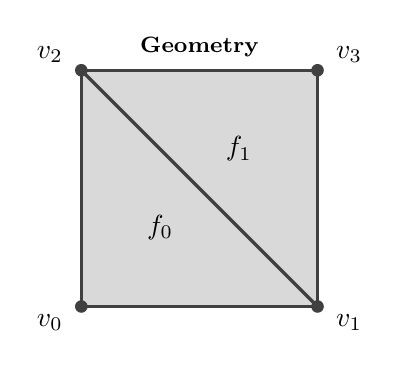
\begin{tikzpicture}[]
            \draw[-, color=darkgray, very thick, fill=darkgray!20]  (0, 0) -- (3, 0) -- (3, 3) -- (0, 3) -- (0, 0) -- (3, 0);
            \draw[-, color=darkgray, very thick]  (0, 3) -- (3, 0);
            \node[fill=darkgray, circle, inner sep=0pt, minimum size=1.6mm] (c) at (0, 0) {};
            \node[fill=darkgray, circle, inner sep=0pt, minimum size=1.6mm] (c) at (3, 0) {};
            \node[fill=darkgray, circle, inner sep=0pt, minimum size=1.6mm] (c) at (0, 3) {};
            \node[fill=darkgray, circle, inner sep=0pt, minimum size=1.6mm] (c) at (3, 3) {};
            \node (x) at (-0.4, -0.2) {$ v_0 $};
            \node (x) at (3.4, -0.2) {$ v_1 $};
            \node (x) at (-0.4, 3.2) {$ v_2 $};
            \node (x) at (3.4, 3.2) {$ v_3 $};
            \node (x) at (1, 1) {$ f_0 $};
            \node (x) at (2, 2) {$ f_1 $};
            \node (x) at (1.5, 3.3) {\bfseries\footnotesize Geometry};
        \end{tikzpicture}
        \caption{}
    \end{subfigure}

    \caption[Example triangle mesh geometry of a two-dimensional square]{
        Example triangle mesh geometry of a two-dimensional square (c), defined using vertex (a), and face (b) lists.}
    \label{fig:Implementation/SceneRepresentation/mesh}
\end{figure}

The high fidelity of triangle meshes renders them a great choice for accurately representing practically any shapes and models.
A diverse array of three-dimensional primitives, such as cubes, spheres, and cones, can easily be modeled using this representation with a controlled level of detail. 
Additionally, triangle meshes provide a straightforward way of calculating surface normals, used throughout ray tracing engines for reflecting rays and shading objects.
Given two non-parallel triangle edges $ |\bm{AB}|, |\bm{BC}| $, the surface normal $ \bm{\hat{n}} $ can be found as the cross product:
%
\begin{equation}
    \bm{\hat{n}} = \frac{|\bm{AB}|\times|\bm{BC}|}{\norm{|\bm{AB}|\times|\bm{BC}|}}
\end{equation}

\subsection{Lights}

Light sources are without a doubt one of the most important concepts in ray tracing, as they contribute to the overall illumination of the rendered scene.
The choice of light types depends on the desired visual effects and the characteristics of the scene being rendered.
In order to effectively illuminate the scene, YART defines two types of light sources: point lights and ambient illumination.
Point lights are often used to represent small, concentrated light sources, such as a light bulb. 
They are generally defined using some intensity value, and a single point in space that emits light uniformly in all directions.
On the other hand, ambient lighting is a basic form of global illumination, which defines the baseline intensity of the scene.
While not a physically accurate light source, it helps to enhance poorly-lit surfaces and areas in shadows. 
As opposed to point lights, ambient lighting does not generate shadows in the rendered image.

\subsection{Materials}\label{ch:Implementation/SceneRepresentation/Materials}

Numerous types of materials can be implemented in ray tracing applications to simulate the appearance of different surfaces.
These can vary between highly realistic, physically based approaches, and simpler, although typically much more efficient, surface shading methods.
YART does not aim to achieve the highest possible levels of realism, and instead puts more effort into being flexible and interactive. 
For this reason, the engine employs diffuse materials with specular highlights, which is a simplistic and easy to implement shading model.
The diffuse shading model (also known as \textit{Lambertian reflectance} \supercite{Goral1984}) is used to model ideal light reflectance scenarios of perfectly matte objects. 
It is based on the Lambert's law, which states that the modelled surface will diffuse incident light equally in all directions, regardless of the observer's angle of view.
Specular reflections are commonly added to diffuse materials, which additionally provide realistic highlights from direct light source reflections.
Together with diffuse shading and an ambient illumination term, the specular reflection model is commonly referred to as the \textit{Blinn-Phong} model \supercite{Blinn1977}.
The output light intensity $ L $ can therefore be defined as a sum of three separate terms -- ambient light $ L_a $, diffuse illumination $ L_d $, and a specular term $ L_s $:
%
\begin{equation}
    L = L_a + L_d + L_s \label{eq:Implementation/SceneRepresentation/lighting}
\end{equation}

The ambient term basically acts as an indirect illumination source in the scene, which defines an object's baseline light intensity.
It is defined using an ambient reflectance value $ k_a $, local to a particular object, and the ambient light intensity $ I_a $, which is globally applied to all scene geometry:
%
\begin{equation}
    L_a = k_a  I_a
\end{equation}

On the other hand, the diffuse reflectance term is determined for a specific light source in the scene.
It produces a matte appearance of rough materials, which scatter light equally in all directions.
Given the surface normal $ \bm{\hat{n}} $, a normalized direction vector $ \bm{\hat{l}}, $ pointing from the point of intersection on the surface to the light source, and the angle $ \theta $ between those vectors, the diffuse term $ L_d $ can be expressed as:
%
\begin{equation}
    L_d = k_d  I_{s} \max(0, \cos{\theta}) = k_d  I_{s} \max(0, \, \bm{\hat{n}} \cdot \bm{\hat{l}} \,),
\end{equation}
%
where $ I_s $ is the light source intensity, a=nd $ k_d $ is the surface's local diffuse coefficient.

Finally, specular reflectance is used to model view-dependant highlights for shiny surfaces.
Similarly to diffuse shading, specular illumination is solved for a given light source. 
The specular term $ L_s $ is given by:
%
\begin{equation}
    L_s = k_s  I_{s} \max(0, \, \bm{\hat{n}} \cdot \bm{\hat{h}} \,),
\end{equation}
%
where $ k_s $ is the object's specular reflectance coefficient, and $ \bm{\hat{h}} $ is a half vector between the direction $ \bm{\hat{l}} $ and a negated ray direction vector $ -\bm{\hat{v}} $:
%
\begin{equation}
    \newcommand{\hvec}{-\bm{\hat{v}} + \bm{\hat{l}} \,}
    \bm{\hat{h}} = \frac{\hvec}{\norm{\hvec}}
\end{equation}

\section{Intersection Testing}

Solving for intersections between rays and subsequent scene objects is an important aspect of the ray tracing process.
For each ray, intersection testing is performed to determine whether it intersects with any object in the scene, yielding the exact position of the hit.
Generally, a single ray must compute intersections for every primitive in the scene, in order to find the closest point of intersection along its path.
Depending on the selected geometric primitives used for representing objects, different intersection algorithms can be employed in a ray tracing system.
A common choice for triangle meshes is the use of the \textit{M{\"o}ller-Trumbore} \supercite{Moller2005} algorithm.
It is a highly efficient, minimal-storage method for determining whether a ray intersects a triangle.
Historically, similar algorithms for solving this problem depended on computing the plane on which the triangle lies, to first check for intersections with that plane, and then test wether the intersection point in inside the triangle edges \supercite{Bogart1988}. 
A clear advantage of the M{\"o}ller-Trumbore algorithm is that the plane equation does not need to be neither computed nor stored, resulting in efficient memory usage for triangle meshes.

Knowing the triangle vertices $ (\bm{V}_0, \bm{V}_1, \bm{V}_2) $, a point on it's surface $ \bm{T}(u, v) $, can be given by:
%
\begin{equation}
    \bm{T}(u, v) = (1 - u - v)\bm{V}_0 + u \bm{V}_1 + v \bm{V}_2,
\end{equation}
%
where $ (u, v) $ are \textit{barycentric coordinates}, used for describing a point in terms of a triangle, which must fulfill $ u \ge 0, v \ge 0 $ and $ u + v \le 1 $.
Intuitively, barycentric coordinates can be thought of as weights of the triangle vertices, with $ w = 1 - u - v $ being the third barycentric coordinate. 
The closer a given barycentric coordinate gets to $ 1 $, the closer the resulting point will rest to its respective vertex.
Solving for intersections between a ray $ \bm{r}(t) $, and a triangle $ \bm{T}(u, v) $, is equivalent to computing  $ \bm{r}(t) = \bm{T}(u, v) $, which, using the ray definition from \cref{eq:Implementation/RayDefinition/ray} yields:
%
\begin{equation}
    \bm{P} + t\bm{\hat{v}} = (1 - u - v)\bm{V}_0 + u \bm{V}_1 + v \bm{V}_2
\end{equation}
%
The above equation can be rearranged, giving:
%
\begin{equation}
    \bm{P} - \bm{V}_0 = -t\bm{\hat{v}} + u(\bm{V}_1 - \bm{V}_0) + v(\bm{V}_2 - \bm{V}_0),
\end{equation}
%
which can further be rewritten into row-column vector multiplication:
%
\begin{equation}
    \begin{bmatrix}
        -\bm{\hat{v}}, & \bm{V}_1 - \bm{V}_0, & \bm{V}_2 - \bm{V}_0
    \end{bmatrix}%
    \begin{bmatrix}
        \; t \; \\ \; u \; \\ \; v \;
    \end{bmatrix} = \bm{P} - \bm{V}_0,
\end{equation}
%
ultimately resulting in a system of linear equations with three unknown scalars: the hit distance $ t $ and barycentric coordinates $ (u, v) $.
To solve this equation, M{\"o}ller and Trumbore, in their original paper, use a technique known in mathematics as the Cramer's rule, which is a formula for solving systems of linear equations in terms of determinants. 
\cref{lst:Implementation/IntersectionTesting/moller_trumbore} demonstrates an example implementation of the M{\"o}ller-Trumbore algorithm, used in YART for efficient ray-triangle intersection testing.

\vfill
\begin{figure}[!ht]
    \lstinputlisting[
        xleftmargin=2em, 
        caption={[Ray-triangle intersection testing using the M{\"o}ller-Trumbore algorithm]
            Ray-triangle intersection testing using the M{\"o}ller-Trumbore algorithm.},
        label={lst:Implementation/IntersectionTesting/moller_trumbore}
    ]{include/listings/ListingMollerTrumbore.cpp}
\end{figure}
\vfill
\clearpage

\section{Shading}

While tracing a ray through the scene, the engine must typically handle two, most important cases: hitting the closest object along the rays path, and when it misses every geometry, effectively extending into infinity.
In the most basic configuration, this condition can be examined by solving for intersections with every single geometric primitive in the scene.
While looping over scene objects, it's important to keep track of the smallest hit distance, in order to find the closest possible point of intersection, for which the pixel will eventually be shaded.

\subsection{Miss Shader}

For scenarios when the ray misses every possible geometry, a specialized procedure of rendering the world's sky is usually implemented. 
Numerous ways of rendering the environment can be employed within a ray tracing system, ranging from solid color and gradient skies, to highly detailed, textured skyboxes. 
This functionality is often referred to as the \textit{miss shader} of a rendering pipeline. 
The core purpose of a miss shader is to sample and return the color of the background for a given ray direction.
For the sake of simplicity, the presented implementation will render solid color skies, which are defined by a singular color value, independent of the ray's direction.
This idea is illustrated in \cref{lst:Implementation/Shading/miss_shader}, with an example \verb|MissShader| method, which simply returns the constant sky color.

\begin{figure}[!ht]
    \lstinputlisting[
        xleftmargin=2em, 
        caption={[Solid color \texttt{MissShader} function implementation]
        Solid color \texttt{MissShader} function implementation.},
        label={lst:Implementation/Shading/miss_shader}
    ]{include/listings/ListingMissShader.cpp}
\end{figure}

\subsection{Closest Hit Shader}

When a ray reaches an object's surface, it consumes the illumination level at that point of intersection, which is eventually used to shade the pixel associated with this ray.
The functionality of calculating this value at the closes intersection point is usually referred to as the \textit{closest hit shader}.
This shader is typically responsible for evaluating materials, calculating lighting, and generating shadows. 
At its core, the closest hit shader employed in the YART engine computes diffuse and specular illumination based on the Blinn-Phong shading model.
The reflectance model described in section \ref{ch:Implementation/SceneRepresentation/Materials}, has been defined for a single light source, whereas our scene might accommodate multiple point lights.
The lighting equation (see \cref{eq:Implementation/SceneRepresentation/lighting}) can easily be modified to reflect this, simply by summing over every $ i $-th light source in the scene:
%
\begin{equation}
    L = L_a + \sum_{i=1}^{N}[(L_d)_i + (L_s)_i]
\end{equation}
%
\cref{lst:Implementation/Shading/hit_shader} presents an example closest hit shader function implementation, which computes Blinn-Phong illumination for a given scene. A \verb|HitPayload| object is additionally employed, which is a lightweight structure used for storying the hit context.

\begin{figure}[!ht]
    \lstinputlisting[
        xleftmargin=2em, 
        caption={[\texttt{ClosestHitShader} function implementation for Blinn-Phong shading]
            \texttt{ClosestHitShader} function implementation for Blinn-Phong shading.},
        label={lst:Implementation/Shading/hit_shader}
    ]{include/listings/ListingClosestHitShader.cpp}
\end{figure}

\addtocontents{toc}{\protect\newpage}
\section{The Ray Tracing Loop}\label{ch:Implementation/RayTracingLoop}

All the methodologies described up until this point aid us in implementing the key component of any ray tracing system -- the ray tracing loop. 
It is the fundamental piece of a rendering pipeline, which binds together all processes related to ray tracing, starting with ray generation and ending with pixel shading.

\cref{lst:Implementation/TheRayTracingLoop/ray_tracing} introduces the ray tracing loop implemented in YART, which at its core renders a given scene, from a particular camera's view, to the specified buffer of pixels.
It first retrieves all ray direction for the given image dimensions, using \verb|Camera| class's \verb|GetRayDirections|, defined in \cref{lst:Implementation/RayGeneration/ray_generation_cache}.
These directions are used to create subsequent \verb|Ray| objects, which originate from the camera's position.
In order to determine if, and where a ray has hit the scene, it is then tested for intersections against every triangular geometry in the scene, iterating thorough all mesh objects and the triangles that define them.
The minimal hit distance is recorded between every iteration, in order to find the closest possible intersection point along the rays path.
When a closer intersection is found than the one currently recorded, information about that hit is stored into a \verb|HitPayload| structure.
This payload can be defined in a multitude of ways, depending on what information is needed for the closest hit shader to shade a surface.
In YART, hit payloads are used to describe the hit object, distance to, and position of the intersection, along with the normal of the intersected surface. 
Finally, the ray tracing loop sets the output image's pixel, to a color returned by either the miss, or closest hit shader, declared respectively in Listings \ref{lst:Implementation/Shading/miss_shader} and \ref{lst:Implementation/Shading/hit_shader}.
\cref{fig:Implementation/TheRayTracingLoop/render} illustrates a sample scene with multiple objects and point lights, rendered using the ray tracing loop described in this section.

\vfill
\begin{figure}[!ht]
    \centering
    \includegraphics[height=9cm]{example-image-b}
    \caption[Sample scene rendered using the basic ray tracing loop]{
        Sample scene rendered using the basic ray tracing loop.}
    \label{fig:Implementation/TheRayTracingLoop/render}
\end{figure}
\vfill

\begin{figure}
    \lstinputlisting[
        xleftmargin=2em, 
        aboveskip=0pt,
        belowskip=0pt,
        caption={[Implementation of YART's ray tracing loop]
            Implementation of YART's ray tracing loop.},
        label={lst:Implementation/TheRayTracingLoop/ray_tracing}
    ]{include/listings/ListingRayTracingLoop.cpp}
\end{figure}\clearpage

\section{Hard Shadows}

The results of the ray tracing loop presented in \cref{ch:Implementation/RayTracingLoop} can be improved in a variety of ways.
One such example is the addition of shadows, which help convey a sense of depth in the final rendered image.
As with any visual effect in rendering engines, shadows can be implemented in a multitude of different ways.
The most straightforward technique involves casting an additional ray for every intersection with the scene, checking whether light is blocked by an object, preventing it from reaching a particular surface.
This methodology is generally referred to as \textit{hard shadows}, due to the characteristic, sharp and well-defined boundaries of shadows generated in resulting renders.
While colliding with an object's surface, a \textit{shadow ray} is additionally traced from the point of intersection, in the direction of a particular light source.
A shadow ray does not evaluate surface illumination nor does it sample the sky's color.
Instead, it only tests for intersections along its path, determining wether a light's path is obstructed by scene geometry.
The core idea behind hard shadows is illustrated in \cref{fig:Implementation/Shadows/shadows}.

\begin{figure}[!ht]
    \centering

    % Path that follows the edges of the current page for clipping
    \tikzstyle{reverseclip}=[insert path={(current page.north east) --
        (current page.south east) --
        (current page.south west) --
        (current page.north west) --
        (current page.north east)}
    ]

    \pgfdeclareradialshading{tikzfadeout}{\pgfpointorigin}{
        color(1.5mm)=(pgftransparent!0); 
        % color(4mm)=(pgftransparent!20); 
        color(9mm)=(pgftransparent!100)
    }
    \pgfdeclarefading{fadeout}{\pgfuseshading{tikzfadeout}}

    \vspace*{1em}
    \begin{tikzpicture}[scale=1.0, every node/.style={scale=1.0}]
        % Plane
        \draw[{Round Cap[length=40pt]}-{Round Cap[length=20pt]}, color=darkgray, very thick] 
            (12.7mm, -55mm) -- (-11.5mm, -40.5mm) -- (53mm, -20.5mm) -- (133mm, -44mm) -- (118mm, -55mm);

        % Shadow
        \draw[darkgray!40, fill=darkgray!40, rotate=85] (-41mm,-74mm) ellipse (13mm and 34mm) {};

        % Camera Lens
        \draw[darkgray, thick] (0,0) ellipse (3mm and 3.6mm);
        \draw[darkgray] (-4.9mm,4.45mm) arc (105:260:3mm and 3.67mm);

        % Camera Body
        \draw[-, color=darkgray, thick] (-0.7mm, -3.5mm) -- (-4.6mm, -2.8mm) -- (-8.7mm, -3.4mm) -- 
            (-8.9mm, 4mm) -- (0.6mm, 5.3mm) -- (-3mm, 6.1mm) -- (-12.7mm, 4.8mm)  -- (-12.4mm, -2.3mm) --
            (-8.7mm, -3.4mm) -- (-8.9mm, 4mm) -- (-12.7mm, 4.8mm);
        \draw[-, color=darkgray, thin] (0.6mm, 3.62mm) -- (-4.7mm, 4.55mm);
        \draw[-, color=darkgray, thick] (1.2mm, 3.4mm) -- (1.2mm, 5.3mm);

        % Sphere
        \node[draw=axis_blue!20!darkgray, very thick, fill=axis_blue!45!gray, circle, inner sep=0pt, minimum size=36mm] (c) at (79.6mm, -20mm) {};

        \begin{scope}
            \begin{pgfinterruptboundingbox}
                \path [clip, rotate=-10] (81mm, 2mm) ellipse (18mm and 10mm) [reverseclip];
            \end{pgfinterruptboundingbox}
            
            \node[draw=axis_blue!20!darkgray, very thick, fill=axis_blue!65, circle, inner sep=0pt, minimum size=36mm] (c) at (79.6mm, -20mm) {};
        \end{scope}

        % Rays background
        \draw[{Round Cap[]}-, color=axis_red, very thick] (0, 0) -- (24.5mm, -0.95mm);
        \draw[{Round Cap[]}-, color=axis_red, very thick] (0, 0) -- (29mm, -18.34mm);

        % Image Plane fill
        \draw[-, color=white!0, fill=white, fill opacity=0.65] (6.8mm, -27.5mm) -- (6.2mm, 6.2mm) --
            (44mm, 11mm) -- (43.3mm, -17.5mm) -- (6.8mm, -27.5mm) -- (6.2mm, 6.2mm);

        \node[draw=axis_blue!20!darkgray, thin, fill=axis_blue!45!gray, circle, inner sep=0pt, minimum size=16mm, rotate=90, xslant=-0.1, fill opacity=0.65, draw opacity=0.65] (c) at (26.3mm, -7mm) {};

        \begin{scope}
            \path[clip, rotate=90, xslant=-0.1] (-9.7mm, -26.3mm) circle (8mm);
            \node[fill=axis_blue!40, circle, inner sep=0pt, minimum size=16mm, rotate=90, xslant=-0.1, fill opacity=0.65, draw opacity=0.0] (c) at (26.5mm, 1mm) {};
        \end{scope}

        \draw[draw=white!0, fill=darkgray!40, circle, inner sep=0pt, minimum size=16mm, fill opacity=0.65, draw opacity=0, rotate=10] (22.3mm, -22.5mm) ellipse (10mm and 3mm) {};

        % Image Plane inner lines 
        \draw[-, color=gray, thin] (12mm, -26mm) -- (11.6mm, 6.8mm);
        \draw[-, color=gray, thin] (17.3mm, -24.7mm) -- (16.9mm, 7.4mm);
        \draw[-, color=gray, thin] (22mm, -23.5mm) -- (21.9mm, 8mm);
        \draw[-, color=gray, thin] (26.8mm, -22.2mm) -- (26.7mm, 8.6mm);
        \draw[-, color=gray, thin] (31.2mm, -21mm) -- (31.2mm, 9.2mm);
        \draw[-, color=gray, thin] (35.2mm, -19.5mm) -- (35.5mm, 9.8mm);
        \draw[-, color=gray, thin] (39.5mm, -18.5mm) -- (39.8mm, 10.4mm);

        \draw[-, color=gray, thin] (6.8mm, -20.6mm) -- (43.5mm, -12mm);
        \draw[-, color=gray, thin] (6.7mm, -14mm) -- (43.5mm, -6.3mm);
        \draw[-, color=gray, thin] (6.5mm, -7.6mm) -- (43.6mm, -0.4mm);
        \draw[-, color=gray, thin] (6.2mm, -0.2mm) -- (44mm, 5.2mm);

        % Image Plane outer lines 
        \draw[-, color=darkgray, very thick] (6.8mm, -27.5mm) -- (6.2mm, 6.2mm) -- (44mm, 11mm) -- 
            (43.3mm, -17.5mm) -- (6.8mm, -27.5mm) -- (6.2mm, 6.2mm);

        % Rays foreground
        \draw[-{Round Cap[]}, color=axis_red, very thick] (29mm, -18.34mm) -- (72.5mm, -45.8mm) -- (74.7mm, -37.3mm);
        \draw[-{Round Cap[]}, color=darkgray, very thick, dashed] (74.7mm, -37.3mm) -- (89.5mm, 19mm);
        \draw[-{Round Cap[]}, color=axis_red, very thick] (24.5mm, -0.95mm) -- (73.5mm, -2.9mm) -- (89.5mm, 19mm);

        % Rays tips
        \draw[-{Latex[length=3mm]}, color=axis_red, ultra thin] (73.5mm, -2.9mm) -- (79.3mm, 5mm);
        \draw[-{Latex[length=3mm]}, color=darkgray, ultra thin] (85.295mm, 3mm) -- (85.35mm, 3.2mm);

        % Light source fading 
        \begin{scope}
            \path[clip] (50mm, 19mm) rectangle (100mm, -30mm);
            \node[fill=white, circle, inner sep=0pt, minimum size=40mm, path fading=fadeout] (c) at (89.5mm, 19mm) {};
        \end{scope}

        % Light source
        \node[fill=white, draw=darkgray, thick, circle, inner sep=0pt, minimum size=3.5mm] (c) at (89.5mm, 19mm) {};

        \foreach\angle in { 0,40,...,360 }{
            \draw[darkgray, thick, rotate around={\angle:(89.5mm, 19mm)}]
                (89.5mm, 21.5mm) -- +(0, 1.5mm);
        }

        % Labels
        \node[color=darkgray] (x) at (-7mm, 10mm) {\textbf{Camera}};
        \node[color=axis_red,rotate=-2] (x) at (57mm, 1mm) {\textbf{Ray}};
        \node[color=darkgray, rotate=6, xslant=0.15] (x) at (25mm, 12mm) {\textbf{Image}};
        \node[color=axis_blue!80, align=left] (x) at (102mm, -8mm) {\textbf{Scene} \\ \textbf{\;\;Object}};
        \node[color=darkgray, align=left] (x) at (103mm, 19mm) {\textbf{Light} \\ \textbf{Source}};

    \end{tikzpicture}
    \vspace*{1em}

    \caption[Simplified model of rendering hard shadows]{
        Simplified model of rendering hard shadows.}
    \label{fig:Implementation/Shadows/shadows}
\end{figure}

The rendering loop introduced in \cref{lst:Implementation/TheRayTracingLoop/ray_tracing} can easily be modified for casting hard shadows. 
Firstly, the functionality of testing for intersections with all scene objects might be extracted from the \verb|RayTrace| method for reuse. 
\cref{lst:Implementation/Shadows/intersect_scene} presents an example \verb|IntersectScene| function, created for this purpose.

\clearpage
\begin{figure}[!ht]
    \lstinputlisting[
        xleftmargin=2em, 
        caption={[\texttt{IntersectScene} method implementation]
            \texttt{IntersectScene} method implementation.},
        label={lst:Implementation/Shadows/intersect_scene}
    ]{include/listings/ListingIntersectScene.cpp}
\end{figure}

Making use of the above function, the \verb|RayTrace| method can be further modified to cast and handle shadow rays. 
\cref{lst:Implementation/Shading/intersect_scene} demonstrates an example implementation reflecting this change.
Shadow rays are traced from a determined point of intersection, in the directions of every light source in the scene. 
When one of these rays collides with an object before reaching a light source, the lights intensity value gets subtracted from a \verb|shadow| variable, which determines how much a surface point is in shadow.
The lower the value of this variable, the less a surface point is lit.
Finally, the output color returned by the closest hit shader is multiplied by this value, effectively darkening specific areas in the output image. 

\clearpage
\begin{figure}
    \lstinputlisting[
        xleftmargin=1.1em, 
        aboveskip=0pt,
        belowskip=0pt,
        caption={[Modification of the ray tracing loop for generating hard shadows]
            Modification of the ray tracing loop for generating hard shadows.},
        label={lst:Implementation/Shading/intersect_scene}
    ]{include/listings/ListingShadows.cpp}
\end{figure}
\clearpage

\cref{fig:Implementation/Shadows/render} illustrates a sample scene with multiple objects and point lights, rendered using the modified ray tracing loop described in this section.

\begin{figure}[!ht]
    \centering
    \includegraphics[height=9cm]{example-image-c}
    \caption[Sample scene rendered using the modified ray tracing loop]{
        Sample scene rendered using the modified ray tracing loop.}
    \label{fig:Implementation/Shadows/render}
\end{figure}
